\chapter{Conclusão}
O trabalho atingiu os objetivos definidos para criação de uma aplicação básica para monitoramento energético na Universidade de Brasília. A aplicação está em um estado funcional, apesar de não ter sido implantada de forma definitiva. Existe uma instância em homologação, sendo executada na infraestrutura do Laboratório Avançado de Pesquisa e Produção de \textit{Software}\footnote{\url{http://lappis.rocks/}} (LAPPIS), presente na Faculdade UnB Gama.

Foi realizada uma apresentação do sistema para os professores de Engenharia de Energia, citados anteriormente no trabalho. Boas críticas foram obtidas para o projeto em si, com ênfase nas medições realizadas e como essas foram apresentadas. Além disso, os professores realizaram comentários para futuras propostas de projetos de eficiência energética em outros órgãos públicos que pudessem utilizar como base o SMI-UnB.

\section{Trabalhos Futuros}
Melhoramentos futuros estão abertos para serem realizados sobre o trabalho, estes são:

\begin{itemize}
    \item Aperfeiçoar \textit{layout da aplicação}
    \item Aprimorar segurança e sincronização da API;
    \item Automatizar ainda mais as tasks para o Docker;
    \item Criar receitas para a aplicação;
    \item Monitoramento de outros recursos (por exemplo, água)
    \item Realizar testes funcionais e de integração;
    \item Realizar testes de usabilidade com usuários finais;
    \item Realizar sistema de \textit{log} que informe as ações realizadas pelos usuários;
    \item Realizar um sistema de \textit{backup};
    \item Realizar a funcionalidade para esquecimento de senhas, via e-mail;
    \item Separar os transdutores numa VLAN segregada para evitar interferências em suas operações;
    \item Subir a imagem do serviço \textit{web} no Docker Hub;
    \item Otimizar as imagens do Docker para ocuparem menos espaço.
\end{itemize}

\section{Cronograma}
Para a realização do cronograma do projeto, Figuras \ref{cronograma} e \ref{cronograma_2}, utilizou-se a ferramenta \textit{Gantter}. Os cronogramas abordam como se dividiram as sprints e atividades realizadas no decorrer do desenvolvimento do SMI-UnB.

\begin{figure}[!htpb]
    \centering
    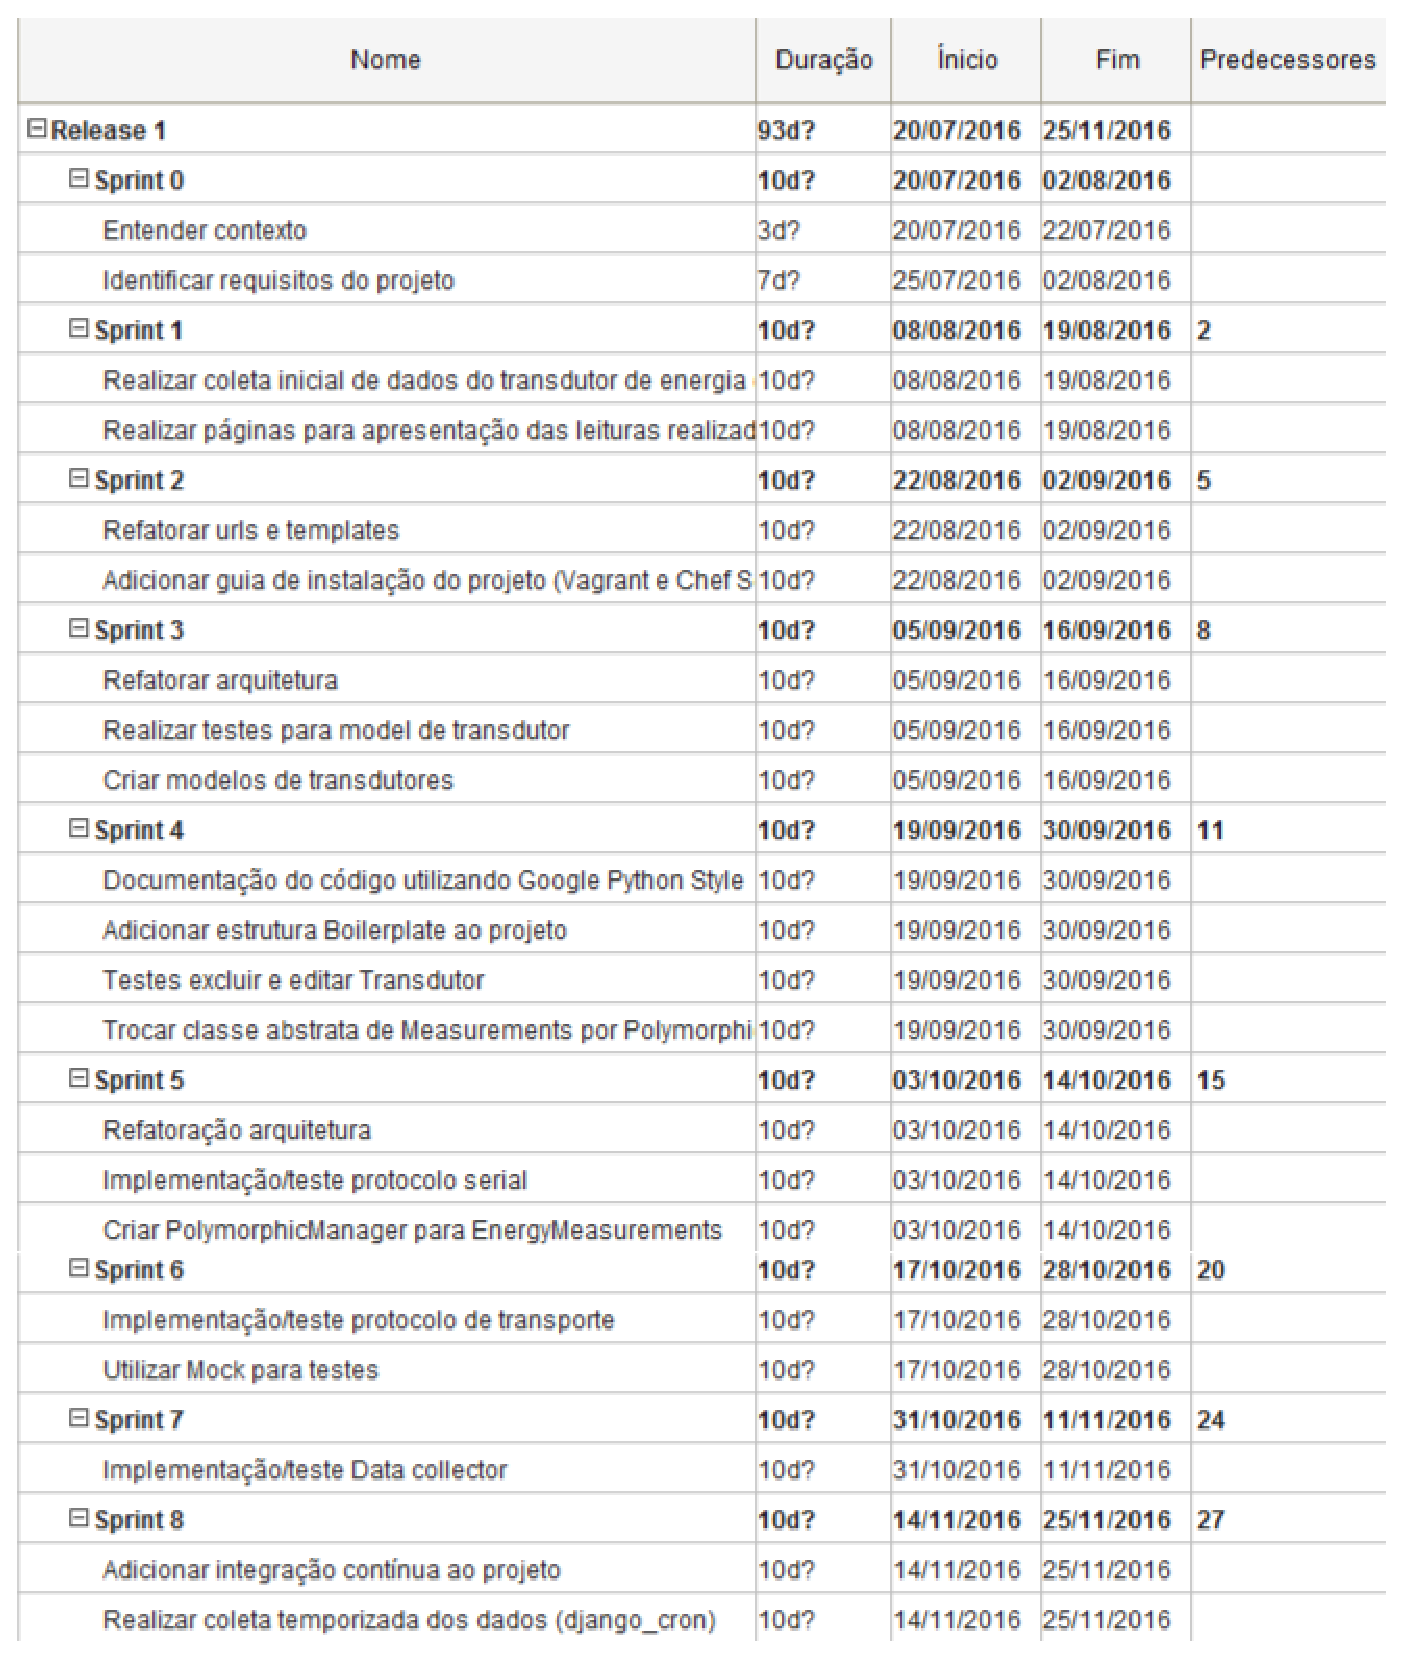
\includegraphics[keepaspectratio=true,scale=0.6]{figuras/cronograma.eps}
    \caption{Cronograma da \textit{release} 1.}
    \label{cronograma}
\end{figure}

\begin{figure}[!htpb]
    \centering
    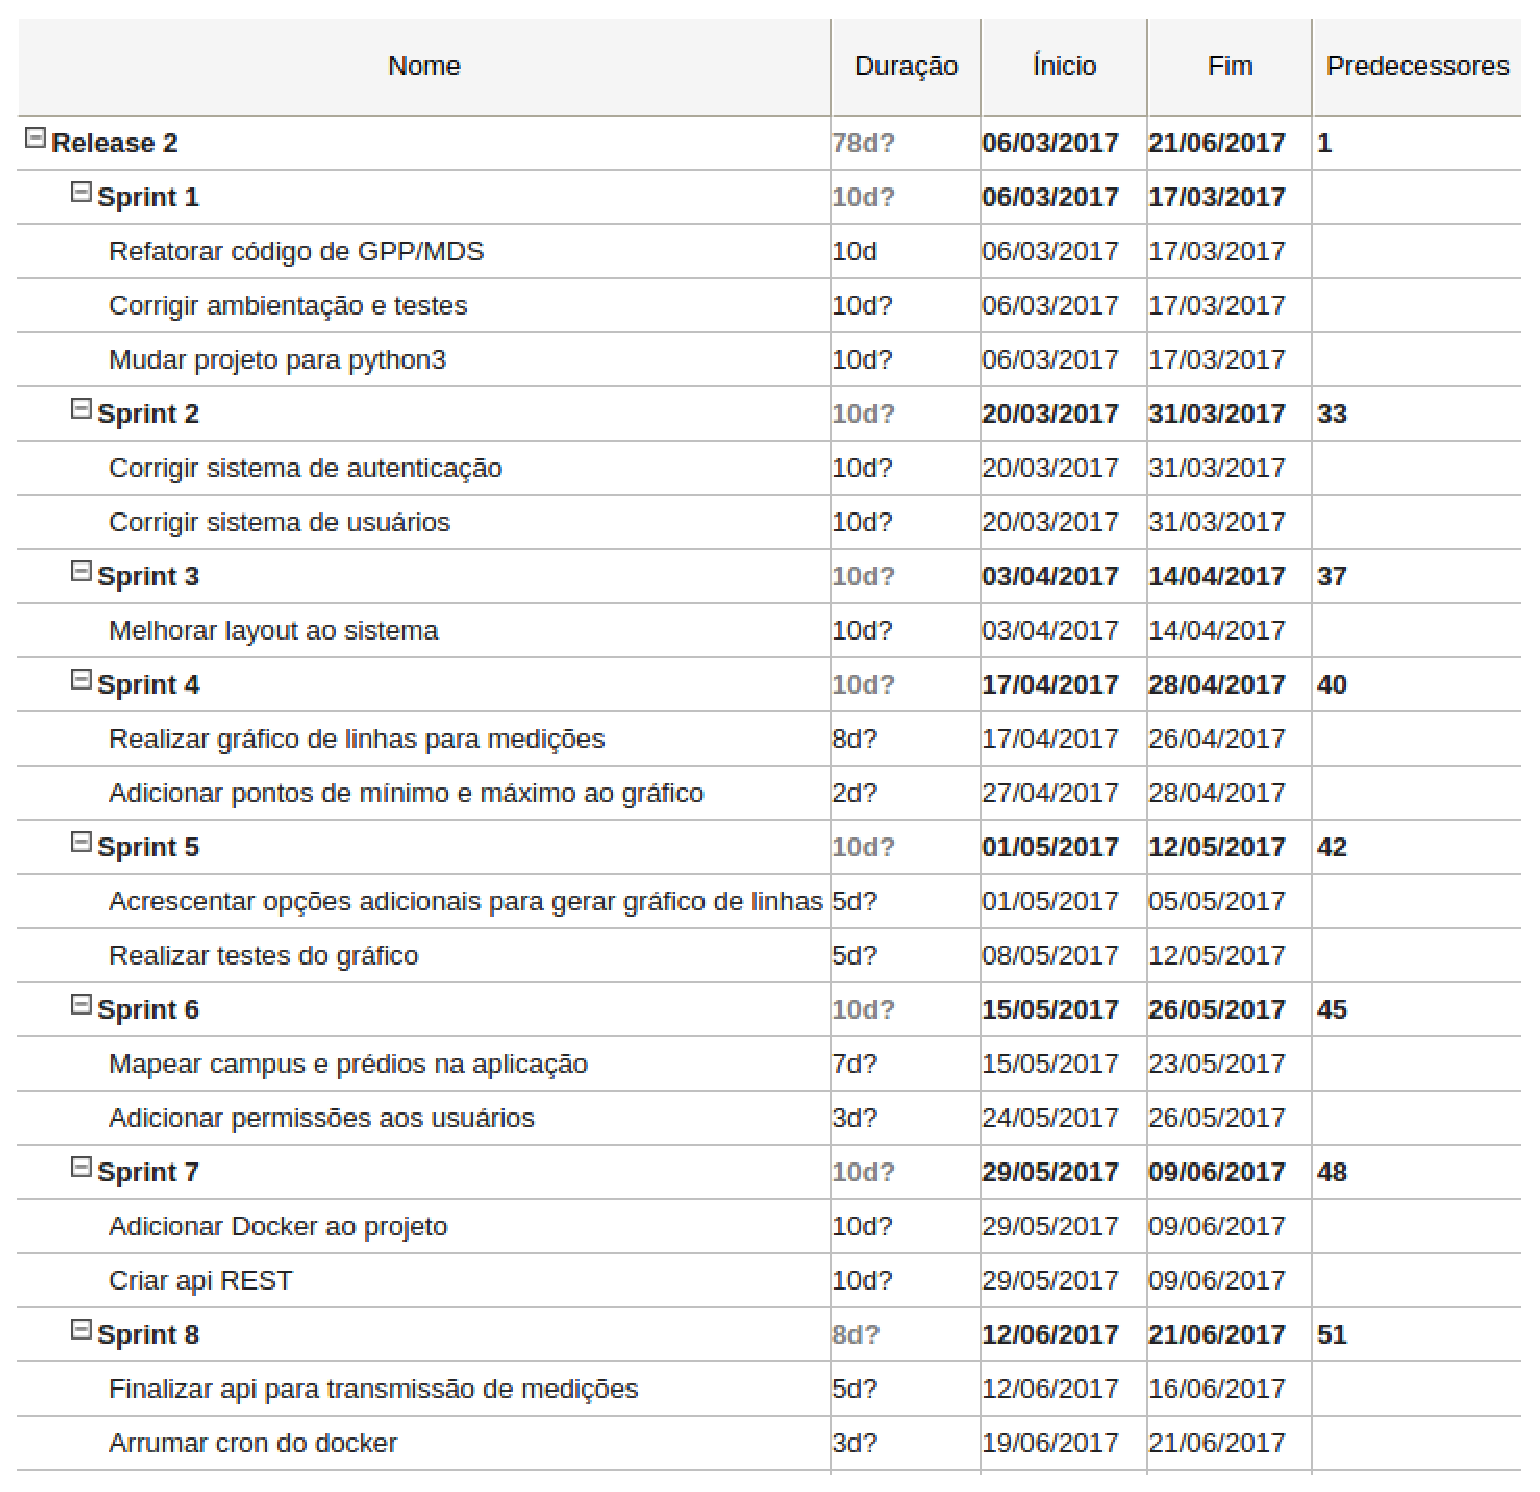
\includegraphics[keepaspectratio=true,scale=0.6]{figuras/cronograma_2.eps}
    \caption{Cronograma da \textit{release} 2.}
    \label{cronograma_2}
\end{figure}